\section{Water vapour channel selection}
%=======================================
Tests assimilating IASI water vapour channel radiances in the GSI indicated that much more data from the higher-peaking channels were making it into the system. This is shown in figure \ref{fig:iasiB2.spc_counts} where a section of the IASI band 2 spectrum is over-plotted with the test assimilation data count. It is quite obvious there is a correlation between high assimilation count and strong absorption lines. This result was thought to be slightly peculiar since knowledge of the water vapour amount at these high levels is not that good.
\begin{figure}[htp]
  \centering
  \includegraphics[scale=0.8]{graphics/wv/iasiB2.spc_counts.eps}
  \caption{A section of an IASI band 2 spectrum in the 6.7\micron{} water vapour region showing the location of the 616 channel subset (red diamonds). The green line shows the number of IASI observations that were assimilated. Note the correlation between strong water vapour absorption and high assimilation count. The vertical magenta lines correspond to channels 3165, 3168, and 3175 with frequencies of 1436.0, 1436.75, and 1438.5\invcm{} respectively.}
  \label{fig:iasiB2.spc_counts}
\end{figure}

In an effort to determine the cause of the correlation shown in figure \ref{fig:iasiB2.spc_counts}, the water vapour Jacobians for selected channels were inspected. The selected channels, indicated via the vertical magenta lines in figure \ref{fig:iasiB2.spc_counts}, correspond to channels 3165, 3168, and 3175 with frequencies of 1436.0 (medium strength line edge absorption), 1436.75 (strong on-line absorption), and 1438.5\invcm{} (weaker, off-line absorption) respectively. The water vapour Jacobians for channels 3165, 3168, and 3175 are shown in figures \ref{fig:IASI_ch3165.TL_K.dTbdLogwLogP} to \ref{fig:IASI_ch3175.TL_K.dTbdLogwLogP}. The most striking feature of these plots is for the channel 3168 Jacobian in figure \ref{fig:IASI_ch3168.TL_K.dTbdLogwLogP} where there is a significant signal above 200hPa.

The next question asked was: ``Are these IASI Jacobians produced by the CRTM correct?'' Chris Barnet's group (NESDIS/STAR) who are developing retrieval algorithms with IASI data and use a different radiative transfer package computed some Jacobians for a similar atmosphere and the results were almost identical. Additionally, AIRS water vapour Jacobians for an on- and off-line channel the same spectral region (see figure \ref{fig:airsM3M4b.spc_subsetloc}) were computed and their characteristics, see figures \ref{fig:AIRS_ch1644.TL_K.dTbdLogwLogP} and \ref{fig:AIRS_ch1652.TL_K.dTbdLogwLogP}, agree with the IASI Jacobians.

It is a known problem that the upper level water vapour background fields in the GDAS are not that good, so why are the strong water vapour channels doing so well with regards to assimilation count? Two possibilities present,
\begin{enumerate}
  \item The upper level water vapour variability is low and most of the error is in the bias, or
  \item These channels peak above clouds so more of them make it past QC.
\end{enumerate}

Regardless of which of these dominate the assimilation count for the strong channels, these strong water vapour channels cannot be effectively used until there is a more useful representation of the upper level water vapour.

\begin{figure}[htp]
  \centering
  \begin{tabular}{c c}
    \multicolumn{2}{c}{$\frac{\displaystyle\partial T_{B}}{\displaystyle\partial\ln(q)}$ \sffamily\textbf{for IASI channel 3165 (1436.0\invcm)}}\\
    {\small\textsf{Tropical}} & {\small\textsf{Midlatitude Summer}}\\
    \includegraphics[bb=90 390 300 565,clip,scale=0.8]{graphics/wv/TL_K/IASI_ch3165.TL_K.dTbdLogwLogP.Model1.eps} &
    \includegraphics[bb=90 390 300 565,clip,scale=0.8]{graphics/wv/TL_K/IASI_ch3165.TL_K.dTbdLogwLogP.Model2.eps} \\
    {\small\textsf{Midlatitude Winter}} & {\small\textsf{Subarctic Summer}}\\
    \includegraphics[bb=90 390 300 565,clip,scale=0.8]{graphics/wv/TL_K/IASI_ch3165.TL_K.dTbdLogwLogP.Model3.eps} &
    \includegraphics[bb=90 390 300 565,clip,scale=0.8]{graphics/wv/TL_K/IASI_ch3165.TL_K.dTbdLogwLogP.Model4.eps} \\
    {\small\textsf{Subarctic Winter}} & {\small\textsf{U.S. Standard}}\\
    \includegraphics[bb=90 390 300 565,clip,scale=0.8]{graphics/wv/TL_K/IASI_ch3165.TL_K.dTbdLogwLogP.Model5.eps} &
    \includegraphics[bb=90 390 300 565,clip,scale=0.8]{graphics/wv/TL_K/IASI_ch3165.TL_K.dTbdLogwLogP.Model6.eps}
  \end{tabular}
  \caption{Comparison of the CRTM tangent-linear (black curve with symbol) and adjoint (red curve) $\partial T_{B}$/$\partial\ln(q)$ water vapour Jacobians for IASI channel 3165 for the six standard climatological profiles. Jacobian units are K.}
  \label{fig:IASI_ch3165.TL_K.dTbdLogwLogP}
\end{figure}

\begin{figure}[htp]
  \centering
  \begin{tabular}{c c}
    \multicolumn{2}{c}{$\frac{\displaystyle\partial T_{B}}{\displaystyle\partial\ln(q)}$ \sffamily\textbf{for IASI channel 3168 (1436.75\invcm)}}\\
    {\small\textsf{Tropical}} & {\small\textsf{Midlatitude Summer}}\\
    \includegraphics[bb=90 390 300 565,clip,scale=0.8]{graphics/wv/TL_K/IASI_ch3168.TL_K.dTbdLogwLogP.Model1.eps} &
    \includegraphics[bb=90 390 300 565,clip,scale=0.8]{graphics/wv/TL_K/IASI_ch3168.TL_K.dTbdLogwLogP.Model2.eps} \\
    {\small\textsf{Midlatitude Winter}} & {\small\textsf{Subarctic Summer}}\\
    \includegraphics[bb=90 390 300 565,clip,scale=0.8]{graphics/wv/TL_K/IASI_ch3168.TL_K.dTbdLogwLogP.Model3.eps} &
    \includegraphics[bb=90 390 300 565,clip,scale=0.8]{graphics/wv/TL_K/IASI_ch3168.TL_K.dTbdLogwLogP.Model4.eps} \\
    {\small\textsf{Subarctic Winter}} & {\small\textsf{U.S. Standard}}\\
    \includegraphics[bb=90 390 300 565,clip,scale=0.8]{graphics/wv/TL_K/IASI_ch3168.TL_K.dTbdLogwLogP.Model5.eps} &
    \includegraphics[bb=90 390 300 565,clip,scale=0.8]{graphics/wv/TL_K/IASI_ch3168.TL_K.dTbdLogwLogP.Model6.eps}
  \end{tabular}
  \caption{Comparison of the CRTM tangent-linear (black curve with symbol) and adjoint (red curve) $\partial T_{B}$/$\partial\ln(q)$ water vapour Jacobians for IASI channel 3168 for the six standard climatological profiles. Jacobian units are K.}
  \label{fig:IASI_ch3168.TL_K.dTbdLogwLogP}
\end{figure}

\begin{figure}[htp]
  \centering
  \begin{tabular}{c c}
    \multicolumn{2}{c}{$\frac{\displaystyle\partial T_{B}}{\displaystyle\partial\ln(q)}$ \sffamily\textbf{for IASI channel 3175 (1438.5\invcm)}}\\
    {\small\textsf{Tropical}} & {\small\textsf{Midlatitude Summer}}\\
    \includegraphics[bb=90 390 300 565,clip,scale=0.8]{graphics/wv/TL_K/IASI_ch3175.TL_K.dTbdLogwLogP.Model1.eps} &
    \includegraphics[bb=90 390 300 565,clip,scale=0.8]{graphics/wv/TL_K/IASI_ch3175.TL_K.dTbdLogwLogP.Model2.eps} \\
    {\small\textsf{Midlatitude Winter}} & {\small\textsf{Subarctic Summer}}\\
    \includegraphics[bb=90 390 300 565,clip,scale=0.8]{graphics/wv/TL_K/IASI_ch3175.TL_K.dTbdLogwLogP.Model3.eps} &
    \includegraphics[bb=90 390 300 565,clip,scale=0.8]{graphics/wv/TL_K/IASI_ch3175.TL_K.dTbdLogwLogP.Model4.eps} \\
    {\small\textsf{Subarctic Winter}} & {\small\textsf{U.S. Standard}}\\
    \includegraphics[bb=90 390 300 565,clip,scale=0.8]{graphics/wv/TL_K/IASI_ch3175.TL_K.dTbdLogwLogP.Model5.eps} &
    \includegraphics[bb=90 390 300 565,clip,scale=0.8]{graphics/wv/TL_K/IASI_ch3175.TL_K.dTbdLogwLogP.Model6.eps}
  \end{tabular}
  \caption{Comparison of the CRTM tangent-linear (black curve with symbol) and adjoint (red curve) $\partial T_{B}$/$\partial\ln(q)$ water vapour Jacobians for IASI channel 3175 for the six standard climatological profiles. Jacobian units are K.}
  \label{fig:IASI_ch3175.TL_K.dTbdLogwLogP}
\end{figure}

\begin{figure}[htp]
  \centering
  \includegraphics[scale=0.8]{graphics/wv/airsM3M4b.spc_subsetloc.eps}
  \caption{A section of an AIRS M3 and M4a spectrum in the 6.7\micron{} water vapour region showing the location of the 281 channel subset (red diamonds). The vertical magenta lines correspond to channels 1644 and 1653 with frequencies of 1437.1703 and 1441.8945\invcm{} respectively. See figure \ref{fig:iasiB2.spc_counts} for comparison with IASI.}
  \label{fig:airsM3M4b.spc_subsetloc}
\end{figure}

\begin{figure}[htp]
  \centering
  \begin{tabular}{c c}
    \multicolumn{2}{c}{$\frac{\displaystyle\partial T_{B}}{\displaystyle\partial\ln(q)}$ \sffamily\textbf{for AIRS channel 1644 (1437.1703\invcm)}}\\
    {\small\textsf{Tropical}} & {\small\textsf{Midlatitude Summer}}\\
    \includegraphics[bb=90 390 300 565,clip,scale=0.8]{graphics/wv/TL_K/AIRS_ch1644.TL_K.dTbdLogwLogP.Model1.eps} &
    \includegraphics[bb=90 390 300 565,clip,scale=0.8]{graphics/wv/TL_K/AIRS_ch1644.TL_K.dTbdLogwLogP.Model2.eps} \\
    {\small\textsf{Midlatitude Winter}} & {\small\textsf{Subarctic Summer}}\\
    \includegraphics[bb=90 390 300 565,clip,scale=0.8]{graphics/wv/TL_K/AIRS_ch1644.TL_K.dTbdLogwLogP.Model3.eps} &
    \includegraphics[bb=90 390 300 565,clip,scale=0.8]{graphics/wv/TL_K/AIRS_ch1644.TL_K.dTbdLogwLogP.Model4.eps} \\
    {\small\textsf{Subarctic Winter}} & {\small\textsf{U.S. Standard}}\\
    \includegraphics[bb=90 390 300 565,clip,scale=0.8]{graphics/wv/TL_K/AIRS_ch1644.TL_K.dTbdLogwLogP.Model5.eps} &
    \includegraphics[bb=90 390 300 565,clip,scale=0.8]{graphics/wv/TL_K/AIRS_ch1644.TL_K.dTbdLogwLogP.Model6.eps}
  \end{tabular}
  \caption{Comparison of the CRTM tangent-linear (black curve with symbol) and adjoint (red curve) $\partial T_{B}$/$\partial\ln(q)$ water vapour Jacobians for AIRS channel 1644 for the six standard climatological profiles. Jacobian units are K. See figure \ref{fig:IASI_ch3168.TL_K.dTbdLogwLogP} for comparison with a similar IASI frequency.}
  \label{fig:AIRS_ch1644.TL_K.dTbdLogwLogP}
\end{figure}

\begin{figure}[htp]
  \centering
  \begin{tabular}{c c}
    \multicolumn{2}{c}{$\frac{\displaystyle\partial T_{B}}{\displaystyle\partial\ln(q)}$ \sffamily\textbf{for AIRS channel 1652 (1441.8945\invcm)}}\\
    {\small\textsf{Tropical}} & {\small\textsf{Midlatitude Summer}}\\
    \includegraphics[bb=90 390 300 565,clip,scale=0.8]{graphics/wv/TL_K/AIRS_ch1652.TL_K.dTbdLogwLogP.Model1.eps} &
    \includegraphics[bb=90 390 300 565,clip,scale=0.8]{graphics/wv/TL_K/AIRS_ch1652.TL_K.dTbdLogwLogP.Model2.eps} \\
    {\small\textsf{Midlatitude Winter}} & {\small\textsf{Subarctic Summer}}\\
    \includegraphics[bb=90 390 300 565,clip,scale=0.8]{graphics/wv/TL_K/AIRS_ch1652.TL_K.dTbdLogwLogP.Model3.eps} &
    \includegraphics[bb=90 390 300 565,clip,scale=0.8]{graphics/wv/TL_K/AIRS_ch1652.TL_K.dTbdLogwLogP.Model4.eps} \\
    {\small\textsf{Subarctic Winter}} & {\small\textsf{U.S. Standard}}\\
    \includegraphics[bb=90 390 300 565,clip,scale=0.8]{graphics/wv/TL_K/AIRS_ch1652.TL_K.dTbdLogwLogP.Model5.eps} &
    \includegraphics[bb=90 390 300 565,clip,scale=0.8]{graphics/wv/TL_K/AIRS_ch1652.TL_K.dTbdLogwLogP.Model6.eps}
  \end{tabular}
  \caption{Comparison of the CRTM tangent-linear (black curve with symbol) and adjoint (red curve) $\partial T_{B}$/$\partial\ln(q)$ water vapour Jacobians for AIRS channel 1652 for the six standard climatological profiles. Jacobian units are K. See figure \ref{fig:IASI_ch3175.TL_K.dTbdLogwLogP} for comparison with a similar IASI frequency.}
  \label{fig:AIRS_ch1652.TL_K.dTbdLogwLogP}
\end{figure}
